% !TeX root = ../paper.tex
% !TeX encoding = UTF-8
% !TeX spellcheck = en_US

\section{Evaluation}\label{sec:evaluation}
  
  \begin{itemize}
    \item What to test? (see testing-strategy)
    \item Testing setup
    \item Tests and results
  \end{itemize}

  \begin{figure}[htbp]
    \centering
%    \includestandalone{pictures/tikz/runtime-vs-ocddiscover}
    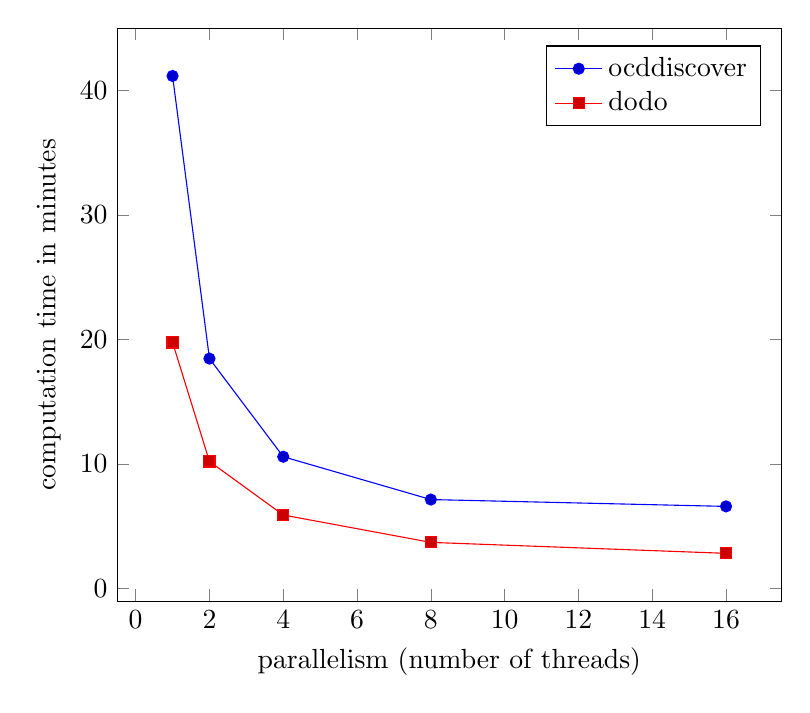
\begin{tikzpicture}
    \begin{axis}[
    scale only axis,
    xlabel=parallelism (number of threads),
    ylabel=computation time in minutes,
    legend pos=north east,
    legend cell align={left},
    ]

    \addplot coordinates {
      (1, 41.17)
      (2, 18.47)
      (4, 10.59)
%      (6, 0.00)
      (8, 7.15)
%      (10, 0.00)
%      (12, 0.00)
%      (14, 0.00)
      (16, 6.60)
    };
    \addplot coordinates {
      (1, 19.77)
      (2, 10.21)
      (4, 5.91)
%      (6, 4.41)
      (8, 3.71)
%      (10, 2.98)
%      (12, 2.98)
%      (14, 2.92)
      (16, 2.83)
    };

    \legend{\gls{ocddiscover}, {\gls{dodo}}}

    \end{axis}
    \end{tikzpicture}
    \caption{Single node runtime comparison of our approach and the baseline algorithm \gls{ocddiscover} with the test dataset \textit{flight\_1k\_stripped\_columns.csv}.}
    \label{fig:runtime-vs-ocddiscover}
  \end{figure}

  \begin{figure}[htbp]
    \centering
    \begin{subfigure}[c]{0.6\textwidth}
      \centering
      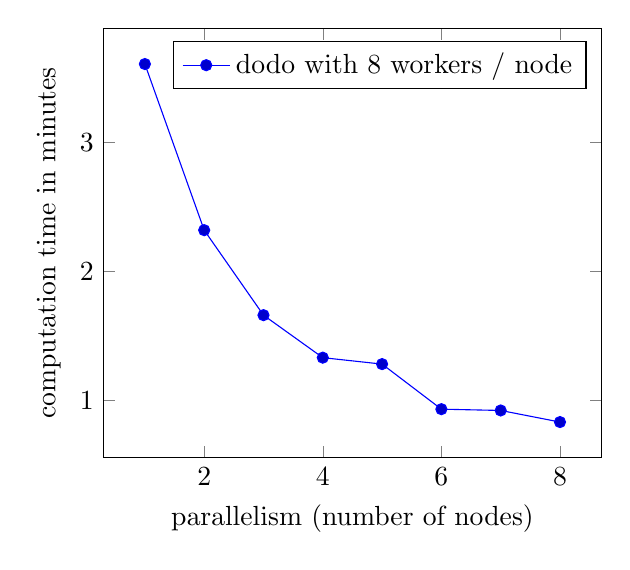
\begin{tikzpicture}[baseline=(current bounding box.center)]
      \begin{axis}[
        scale only axis,
        scale=0.75,
        xlabel=parallelism (number of nodes),
        ylabel=computation time in minutes,
        legend pos=north east,
        legend cell align={left},
      ]

      \addplot coordinates {
        (1, 3.61)
        (2, 2.32)
        (3, 1.66)
        (4, 1.33)
        (5, 1.28)
        (6, 0.93)
        (7, 0.92)
        (8, 0.83)
      };

      \legend{{\gls{dodo} with 8 workers / node}}

      \end{axis}
      \end{tikzpicture}
      \caption{Computation time plottet over the number of nodes.}
      \label{fig:fig:node-scaling}
    \end{subfigure}
    \begin{subtable}[c]{0.39\textwidth}
      \centering
      \begin{tabular}{cr}
        \toprule
        \textbf{\# nodes} & \textbf{computation time} \\
        \midrule
        1 & 3~m~37~s \\
        2 & 2~m~19~s \\
        3 & 1~m~40~s \\
        4 & 1~m~20~s \\
        5 & 1~m~17~s \\
        6 & 56~s \\
        7 & 55~s \\
        8 & 50~s \\
        \bottomrule
      \end{tabular}
      \caption{Computation time for finding all \glspl{od} in the dataset.}
      \label{fig:tab:node-scaling}
    \end{subtable}
    \caption{Scaling our algorithm over the number of nodes and keeping the number of workers fixed using the test dataset \textit{flight\_1k\_stripped\_columns.csv}.}
    \label{fig:node-scaling}
  \end{figure}